\chapter{Literature Review}
\label{ch:literature_review}

This chapter examines two approaches to energy assessment when official building information is incomplete. The first estimates explicit building attributes that can be used for archetype assignment, while the second predicts registered energy classes directly from imagery. Section~\ref{sec:building_attributes_archetype_assignment} first establishes how building attributes affect archetype assignment and thermal calculations. Section~\ref{sec:building_attribute_enrichment} then reviews how missing attributes are estimated from administrative, contextual, geospatial, and image data. Section~\ref{sec:direct_image_energy_class} examines direct energy class prediction from imagery. Section~\ref{sec:comparative_synthesis} compares the information retained and the validation evidence provided by the two approaches, leading to the research gap addressed in this study.

\section{Building Attributes and Archetype Assignment}
\label{sec:building_attributes_archetype_assignment}

Building type and construction year perform different but complementary roles in TABULA archetype assignment. Building age, construction type, size, geometry, use, and technical systems are commonly used to group buildings with similar energy-related characteristics \parencite{reinhart2016,shen_archetype_2024}. Within the Dutch TABULA typology, building type determines the dwelling type category, such as detached, terraced, or apartment buildings, while construction year determines the construction period associated with prevailing construction practices and thermal regulations \parencite{loga2016,rvo2011}. Each combination of dwelling type and construction period defines a separate archetype cell. Accurate cell assignment therefore requires both attributes to be identified correctly. Floor count does not determine the TABULA cell in this study and is evaluated separately as an additional input to energy class prediction.

Assigning a building to a TABULA cell determines which representative thermal properties are used in subsequent heat transmission calculations. These properties include representative U-values for walls, roofs, floors, and windows rather than measurements of the individual building, as shown in Figure~\ref{fig:tabula_u_value} \parencite{loga2016}. A U-value expresses heat flow through a building element per unit area and per degree of temperature difference. ISO 13789 defines steady-state transmission and ventilation heat transfer coefficients for whole buildings and building parts \parencite{iso13789}. Construction period therefore affects the representative thermal properties assigned to a building, while geometry determines the areas over which transmission occurs. Building type is also related to geometric exposure because a detached house generally has more external wall area relative to its volume than a terraced or multifamily building \parencite{wurm2021}. Archetype accuracy must therefore be evaluated not only as a categorical match but also through the change in thermal properties assigned to the building.

\begin{figure}[htbp]
	\centering
	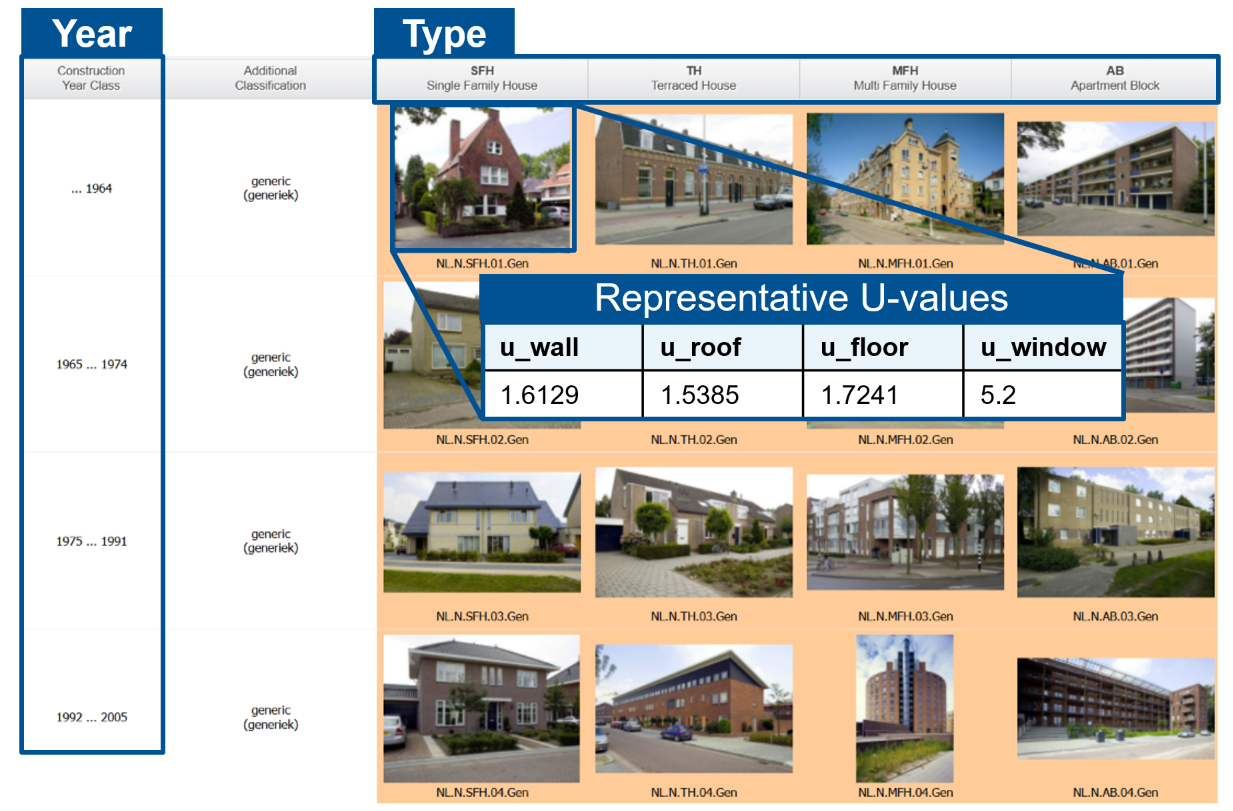
\includegraphics[width=\textwidth]{figures/fig/fig_2_1_tabula_u_value}
	\caption{Building type and construction year determine the archetype cell, from which representative U-values are assigned for heat transmission calculations. Adapted from the TABULA WebTool \parencite{tabulawebtool}.}
	\label{fig:tabula_u_value}
\end{figure}

Evidence from different urban energy modelling contexts shows that uncertainty in building type and construction year can affect energy estimates for individual buildings. In a heat demand model for Hamburg, \textcite{dochev2020} showed that archetype classification based on cadastral construction type and construction epoch could constitute a substantial source of error. The resulting estimates remained plausible at aggregated spatial scales despite discrepancies for individual buildings. Using an urban building energy model covering 50,843 buildings in the United States, \textcite{bass2022} similarly identified estimated building type and construction year as important sources of bias when simulated electricity use was compared with measurements. Although the two studies used different archetype systems and energy outcomes, both found that uncertainty in type and year affected the properties assigned to individual buildings. These findings establish the need to compare reference and estimated attributes at the level of individual buildings before interpreting their aggregate energy effects.

\section{Building Attribute Enrichment}
\label{sec:building_attribute_enrichment}

This section examines how building type, construction year, and related attributes are obtained when complete reference records are unavailable. Existing methods draw on two main sources of evidence. Contextual and geospatial approaches estimate attributes from census records, building morphology, and remote sensing, whereas image approaches use visible characteristics of individual buildings. Image methods also differ in how extensively the selected model is adapted to the target dataset.

\subsection{Administrative, Census, and Geospatial Data}
\label{sec:administrative_geospatial_data}

Administrative and open geospatial datasets improve access to building information but do not consistently provide the attributes required for archetype assignment. Building age information used in urban energy applications varies in availability and level of detail across regions \parencite{garbasevschi2021}. \Ac{OSM} provides broad geographic coverage, but its building descriptions and attribute availability vary between locations. EUBUCCO v0.1 harmonises available footprints and attributes for approximately 202 million buildings across the European Union and Switzerland, yet construction year and building type are available for only 24\% and 46\% of the buildings, respectively \parencite{milojevicdupont2023}. These datasets expand the spatial coverage of building footprints, but they do not eliminate gaps in the information needed to assign individual buildings to archetypes.

When attributes are unavailable, census data and characteristics of buildings and their surroundings can be used to estimate them for individual buildings. \textcite{dabrock2025} trained XGBoost, a gradient boosted tree method, with census, morphological, and socioeconomic features to estimate residential size class and construction year across Germany. The estimated attributes were assigned to TABULA archetypes and evaluated through an individual building test set and comparisons with statistics aggregated by federal state. \textcite{garbasevschi2021} used building characteristics together with street and urban block measures to estimate residential building age across eight German municipalities and then examined the effect of age classification errors on calculated heat demand. Dabrock et al. emphasised nationwide data completion and archetype assignment, whereas Garbasevschi et al. examined how spatial context affected age estimation and its energy consequences. Combining census data with building and neighbourhood characteristics can therefore support attribute estimation over large areas, but the resulting estimates remain dependent on the spatial resolution and composition of the source data.

Remote sensing can provide geometry and morphology at the level of individual buildings and connect the estimated information to an energy model. \textcite{wurm2021} combined aerial imagery and a digital surface model to derive building footprints and heights for approximately 14,800 residential buildings in M\"unster. Morphometric features were used to classify construction type, while census data supplied construction period. The resulting building information was used for heat demand modelling and compared with reference values from the Energy Atlas at a spatial resolution of 100 m. This workflow demonstrates that information derived from remote sensing can enter an energy model, although validation at an aggregated grid level does not isolate the effect of each estimated attribute for the same buildings.

Administrative, census, and geospatial approaches can therefore cover large building stocks and may support archetype assignment or heat demand modelling. Their evidence is nevertheless distributed across different observation and validation levels. Some inputs describe individual buildings, while others describe census cells, urban blocks, or larger administrative units. Consequently, the reported results do not provide a common comparison of all attributes required by one archetype workflow against official values for the same buildings.

\subsection{SVI Based Attribute Estimation}
\label{sec:street_view_attribute_estimation}

\Ac{SVI} offers a different basis for attribute estimation because it depicts the facade of an individual building rather than the statistical context of an area. The images can reveal building form, floor count, facade material, and visual indications of construction period. They provide less direct evidence about insulation, technical systems, or refurbishment that is not visible on the facade. Occlusion, camera position, and image coverage further determine which building characteristics can be observed. \Ac{SVI} therefore provides direct visual evidence for individual buildings, but only for attributes expressed in their visible exterior.

Existing studies show that \ac{SVI} can support both multiattribute enrichment and focused age estimation. \textcite{liang2025} introduced OpenFACADES and used 31,180 crowdsourced Mapillary images from seven cities to estimate building use, surface material, construction year, and floor count. The authors compared convolutional neural networks, vision transformers, and \acp{VLM} using labels assembled primarily from \ac{OSM}, with missing information supplemented from other sources, and then applied the selected framework to a larger image collection. The estimated attributes were not subsequently evaluated in an archetype or energy application. Focusing on construction age, \textcite{zeng2024} used GPT-4 Vision to classify London facade images into construction epochs without updating the model parameters and reported an accuracy of 39.69\%. Liang et al. estimated several building attributes, whereas Zeng et al. considered construction age alone, but neither study evaluated the effect of attribute errors on TABULA assignment or thermal properties. These studies establish the feasibility of estimating energy-related attributes from facade images but do not determine whether the estimates preserve the archetype associated with official records.

\subsection{Image Model Configurations}
\label{sec:image_model_configurations}

The reviewed image methods also differ in how much the model is adapted to local building labels. ResNet-50 is a residual convolutional neural network introduced by \textcite{he2016}. In this study, all pretrained ResNet-50 parameters are updated using labelled images from the target task. DINOv2 provides pretrained visual representations that can remain fixed while supervised prediction heads are trained on local labels \parencite{oquab2023}. InternVL3 is a \ac{VLM} designed to process visual inputs and textual instructions \parencite{zhu2025}. In this study, the released InternVL3 model is used without additional parameter updates to generate building attribute estimates. These configurations therefore represent full adaptation, supervised prediction from a fixed visual representation, and inference through textual instructions using a fixed multimodal model.

The configurations differ in their use of labelled data, computational requirements, and dependence on prior visual knowledge. Results reported in separate studies cannot identify the most suitable configuration for building attribute enrichment because the datasets, attribute definitions, geographic contexts, and evaluation procedures also differ. Their suitability can therefore be compared only when the buildings, labels, image selection procedure, and data partitions are held constant.

\section{Direct Image Based Energy Class Prediction}
\label{sec:direct_image_energy_class}

This section examines a different prediction task in which imagery is mapped directly to a registered energy class without producing explicit building attributes. Using official \ac{EPC} records as labels, \textcite{mayer2023uk} combined \ac{SVI}, aerial imagery, building footprints, and land surface temperature data for 39,605 buildings across four areas in England. The study grouped classes A to D and E to G into a binary task, for which the complete multimodal model achieved a macro F1 score of 64.64\%. \textcite{mayer2023dk} applied the same class grouping to 21,593 buildings in the Copenhagen metropolitan area and reported a macro F1 score of 58.79\% for the combined image model. \Ac{SVI} provided more useful information than aerial imagery in Copenhagen, although the two image sources alone were considered insufficient for reliable classification. Together, the studies show that exterior imagery contains information associated with registered energy performance, but that the available signal depends on the image source and supporting data.

Subsequent studies extended direct prediction by adding structured information or additional sensing modalities. \textcite{liu2025} combined \ac{SVI} from Google Street View with geographic information system attributes and adapted the model with local samples to predict energy classes A to G. \textcite{sun2026} integrated \ac{SVI} with thermal infrared imagery, optical remote sensing, building morphology, and socioeconomic information for binary classification of building energy performance. Related work has also examined zero-shot visual assessment at the building component level. \textcite{pan_nd} evaluated GPT-4o on \ac{SVI} to predict \ac{EPC}-derived wall energy efficiency ratings without updating the model parameters for the target task. This prediction target differs from the \ac{EPC} bands assigned to whole buildings in the studies above. Together, these studies extend image based energy assessment through contextual attributes, additional observations of the building and its surroundings, and knowledge retained by a pretrained multimodal model. The image sources, supporting data, and prediction targets differ across studies.

The reported results therefore cannot be interpreted as direct performance comparisons. The studies differ in class grouping, supporting data, study area, model adaptation, and evaluation protocol. Direct prediction also produces an energy class without retaining estimates of building type, construction year, floor count, or archetype parameters. It can provide an alternative source of energy class information, but it cannot establish whether the corresponding building attributes or archetype assignment are correct.

\section{Comparative Synthesis and Research Gap}
\label{sec:comparative_synthesis}

Attribute enrichment and direct image based energy class prediction retain different information, as shown in Figure~\ref{fig:literature_synthesis}. They also differ in the point at which official reference data enter the evaluation. Attribute enrichment retains estimates of specific building attributes, such as building type, construction year, and floor count, but the attributes included, reference labels, and validation levels vary across studies \parencite{dabrock2025,wurm2021,garbasevschi2021,liang2025,zeng2024}. Studies that predict \ac{EPC} bands directly use registered energy classes as targets but do not retain the intermediate building attributes or thermal parameters \parencite{mayer2023uk,mayer2023dk,liu2025,sun2026}. The Dutch study by \textcite{hettinga2023} shows what can be achieved when official building attributes, reconstructed geometry, neighbourhood information, and registered energy classes can be linked for individual buildings. Its random forest classifier achieved 71\% exact energy class accuracy and 93\% accuracy within one class on a test subset, while TABULA assignment achieved 26\% exact accuracy and 67\% accuracy within one class on the complete certificate dataset. The results were obtained from different evaluation populations and class ranges and therefore do not constitute a controlled comparison between the two methods.

\begin{figure}[htbp]
	\centering
	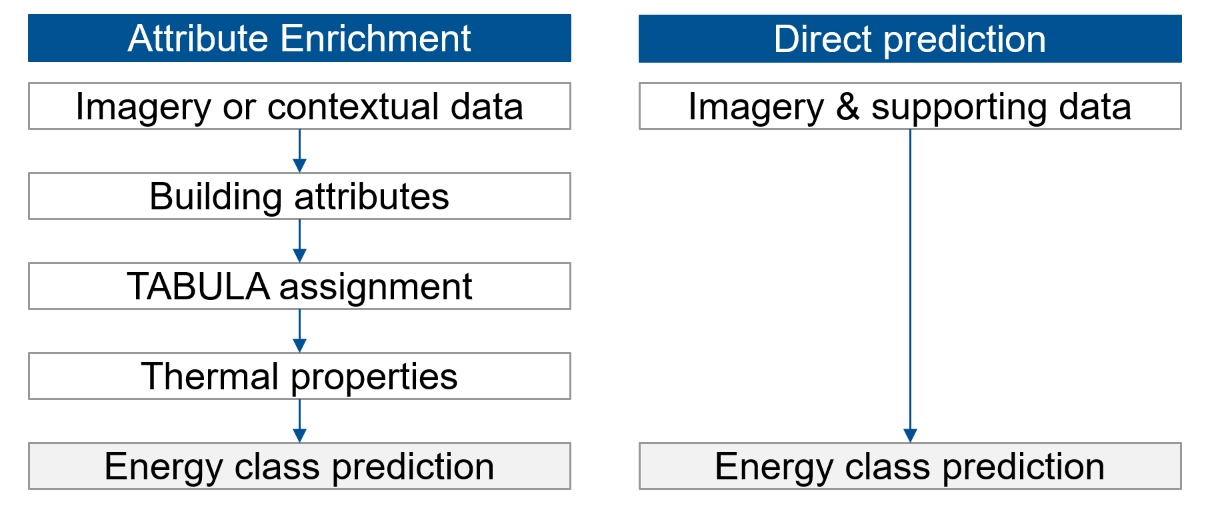
\includegraphics[width=\textwidth]{figures/fig/fig_2_2_synthesis}
	\caption{Comparison of attribute enrichment and direct image based energy class prediction workflows.}
	\label{fig:literature_synthesis}
\end{figure}

The reviewed literature therefore leaves three connected comparisons unresolved. First, estimates of building type, construction year, and floor count have not been jointly compared with official values for the same buildings under common evaluation conditions. Second, the effects of errors in estimated building type and construction year on joint TABULA cell assignment and the associated thermal properties have not been evaluated for those buildings. Third, energy class predictions based on official building attributes, building attributes estimated from imagery, and imagery alone have not been compared using the same buildings, target definitions, data partitions, and evaluation conditions. Addressing these gaps requires a dataset in which imagery, official building attributes, reconstructed geometry, and registered energy classes refer to the same buildings.

Related work has combined geospatial observations, archetype assumptions, and EnergyPlus simulations to construct a synthetic dataset for training graph neural networks to predict energy use intensity \parencite{dalach2026}. Its prediction targets consist of simulation outputs rather than registered energy classes linked to official building attributes. Semi-synthetic data construction is therefore an implementation strategy for the present study rather than a separate literature approach.
